\documentclass[twoside]{book}

% Packages required by doxygen
\usepackage{fixltx2e}
\usepackage{calc}
\usepackage{doxygen}
\usepackage[export]{adjustbox} % also loads graphicx
\usepackage{graphicx}
\usepackage[utf8]{inputenc}
\usepackage{makeidx}
\usepackage{multicol}
\usepackage{multirow}
\PassOptionsToPackage{warn}{textcomp}
\usepackage{textcomp}
\usepackage[nointegrals]{wasysym}
\usepackage[table]{xcolor}

% Font selection
\usepackage[T1]{fontenc}
\usepackage[scaled=.90]{helvet}
\usepackage{courier}
\usepackage{amssymb}
\usepackage{sectsty}
\renewcommand{\familydefault}{\sfdefault}
\allsectionsfont{%
  \fontseries{bc}\selectfont%
  \color{darkgray}%
}
\renewcommand{\DoxyLabelFont}{%
  \fontseries{bc}\selectfont%
  \color{darkgray}%
}
\newcommand{\+}{\discretionary{\mbox{\scriptsize$\hookleftarrow$}}{}{}}

% Page & text layout
\usepackage{geometry}
\geometry{%
  a4paper,%
  top=2.5cm,%
  bottom=2.5cm,%
  left=2.5cm,%
  right=2.5cm%
}
\tolerance=750
\hfuzz=15pt
\hbadness=750
\setlength{\emergencystretch}{15pt}
\setlength{\parindent}{0cm}
\setlength{\parskip}{3ex plus 2ex minus 2ex}
\makeatletter
\renewcommand{\paragraph}{%
  \@startsection{paragraph}{4}{0ex}{-1.0ex}{1.0ex}{%
    \normalfont\normalsize\bfseries\SS@parafont%
  }%
}
\renewcommand{\subparagraph}{%
  \@startsection{subparagraph}{5}{0ex}{-1.0ex}{1.0ex}{%
    \normalfont\normalsize\bfseries\SS@subparafont%
  }%
}
\makeatother

% Headers & footers
\usepackage{fancyhdr}
\pagestyle{fancyplain}
\fancyhead[LE]{\fancyplain{}{\bfseries\thepage}}
\fancyhead[CE]{\fancyplain{}{}}
\fancyhead[RE]{\fancyplain{}{\bfseries\leftmark}}
\fancyhead[LO]{\fancyplain{}{\bfseries\rightmark}}
\fancyhead[CO]{\fancyplain{}{}}
\fancyhead[RO]{\fancyplain{}{\bfseries\thepage}}
\fancyfoot[LE]{\fancyplain{}{}}
\fancyfoot[CE]{\fancyplain{}{}}
\fancyfoot[RE]{\fancyplain{}{\bfseries\scriptsize Generated by Doxygen }}
\fancyfoot[LO]{\fancyplain{}{\bfseries\scriptsize Generated by Doxygen }}
\fancyfoot[CO]{\fancyplain{}{}}
\fancyfoot[RO]{\fancyplain{}{}}
\renewcommand{\footrulewidth}{0.4pt}
\renewcommand{\chaptermark}[1]{%
  \markboth{#1}{}%
}
\renewcommand{\sectionmark}[1]{%
  \markright{\thesection\ #1}%
}

% Indices & bibliography
\usepackage{natbib}
\usepackage[titles]{tocloft}
\setcounter{tocdepth}{3}
\setcounter{secnumdepth}{5}
\makeindex

% Hyperlinks (required, but should be loaded last)
\usepackage{ifpdf}
\ifpdf
  \usepackage[pdftex,pagebackref=true]{hyperref}
\else
  \usepackage[ps2pdf,pagebackref=true]{hyperref}
\fi
\hypersetup{%
  colorlinks=true,%
  linkcolor=blue,%
  citecolor=blue,%
  unicode%
}

% Custom commands
\newcommand{\clearemptydoublepage}{%
  \newpage{\pagestyle{empty}\cleardoublepage}%
}

\usepackage{caption}
\captionsetup{labelsep=space,justification=centering,font={bf},singlelinecheck=off,skip=4pt,position=top}

%===== C O N T E N T S =====

\begin{document}

% Titlepage & ToC
\hypersetup{pageanchor=false,
             bookmarksnumbered=true,
             pdfencoding=unicode
            }
\pagenumbering{alph}
\begin{titlepage}
\vspace*{7cm}
\begin{center}%
{\Large My Project }\\
\vspace*{1cm}
{\large Generated by Doxygen 1.8.14}\\
\end{center}
\end{titlepage}
\clearemptydoublepage
\pagenumbering{roman}
\tableofcontents
\clearemptydoublepage
\pagenumbering{arabic}
\hypersetup{pageanchor=true}

%--- Begin generated contents ---
\chapter{Closet\+Plus\+Plus}
\label{md_README}
\Hypertarget{md_README}
Clone the repo

run {\ttfamily make}

run {\ttfamily ./\+Closet++}

follow prompts 
\chapter{Hierarchical Index}
\section{Class Hierarchy}
This inheritance list is sorted roughly, but not completely, alphabetically\+:\begin{DoxyCompactList}
\item \contentsline{section}{Closet}{\pageref{classCloset}}{}
\item \contentsline{section}{Clothes}{\pageref{classClothes}}{}
\begin{DoxyCompactList}
\item \contentsline{section}{Belt}{\pageref{classBelt}}{}
\item \contentsline{section}{Pants}{\pageref{classPants}}{}
\item \contentsline{section}{Shirt}{\pageref{classShirt}}{}
\item \contentsline{section}{Shoes}{\pageref{classShoes}}{}
\item \contentsline{section}{Socks}{\pageref{classSocks}}{}
\end{DoxyCompactList}
\item \contentsline{section}{Window}{\pageref{classWindow}}{}
\begin{DoxyCompactList}
\item \contentsline{section}{Vulkan}{\pageref{classVulkan}}{}
\end{DoxyCompactList}
\end{DoxyCompactList}

\chapter{Class Index}
\section{Class List}
Here are the classes, structs, unions and interfaces with brief descriptions\+:\begin{DoxyCompactList}
\item\contentsline{section}{\mbox{\hyperlink{classBelt}{Belt}} }{\pageref{classBelt}}{}
\item\contentsline{section}{\mbox{\hyperlink{classCloset}{Closet}} }{\pageref{classCloset}}{}
\item\contentsline{section}{\mbox{\hyperlink{classClothes}{Clothes}} }{\pageref{classClothes}}{}
\item\contentsline{section}{\mbox{\hyperlink{classPants}{Pants}} }{\pageref{classPants}}{}
\item\contentsline{section}{\mbox{\hyperlink{classShirt}{Shirt}} }{\pageref{classShirt}}{}
\item\contentsline{section}{\mbox{\hyperlink{classShoes}{Shoes}} }{\pageref{classShoes}}{}
\item\contentsline{section}{\mbox{\hyperlink{classSocks}{Socks}} }{\pageref{classSocks}}{}
\item\contentsline{section}{\mbox{\hyperlink{classVulkan}{Vulkan}} }{\pageref{classVulkan}}{}
\item\contentsline{section}{\mbox{\hyperlink{classWindow}{Window}} }{\pageref{classWindow}}{}
\end{DoxyCompactList}

\chapter{Class Documentation}
\hypertarget{classBelt}{}\section{Belt Class Reference}
\label{classBelt}\index{Belt@{Belt}}
Inheritance diagram for Belt\+:\begin{figure}[H]
\begin{center}
\leavevmode
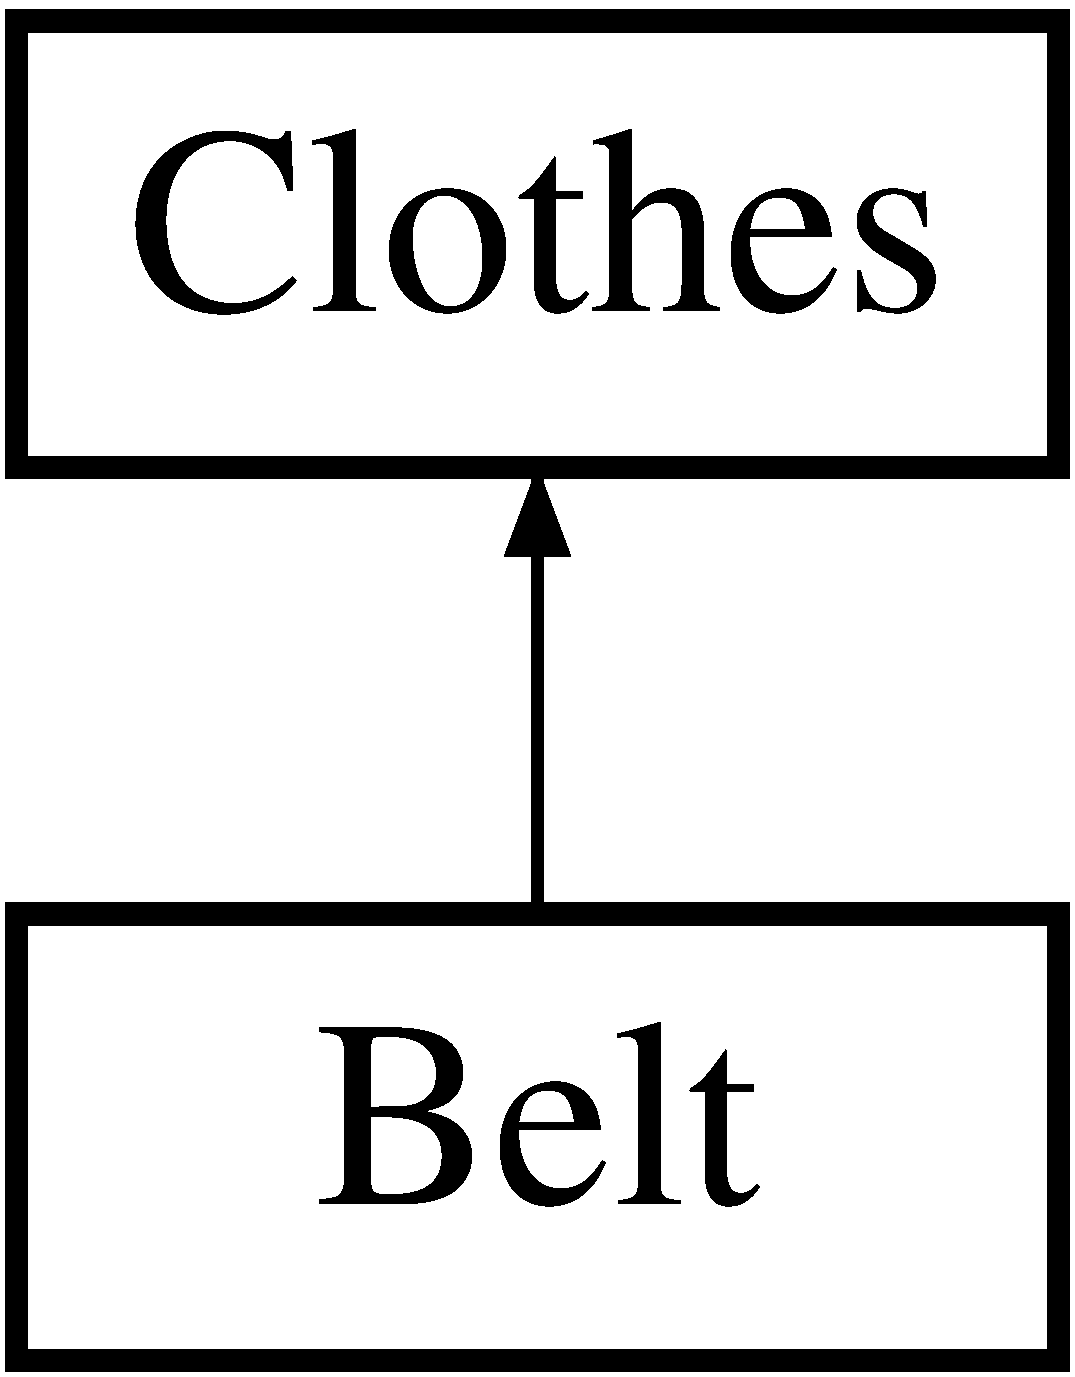
\includegraphics[height=2.000000cm]{classBelt}
\end{center}
\end{figure}
\subsection*{Public Member Functions}
\begin{DoxyCompactItemize}
\item 
\mbox{\Hypertarget{classBelt_a2a8b481a0fe80916513dbd5cf1f03127}\label{classBelt_a2a8b481a0fe80916513dbd5cf1f03127}} 
{\bfseries Belt} (int id, string name, string prim\+\_\+color, string sec\+\_\+color, string tert\+\_\+color, string material, string pattern)
\item 
\mbox{\Hypertarget{classBelt_a69b84739e63f35afa5dacf6f3ce0d731}\label{classBelt_a69b84739e63f35afa5dacf6f3ce0d731}} 
string {\bfseries To\+X\+ML} () const
\item 
\mbox{\Hypertarget{classBelt_af09e2b5e51b7603ec5dede2e6b0a753f}\label{classBelt_af09e2b5e51b7603ec5dede2e6b0a753f}} 
string {\bfseries To\+String} () const
\end{DoxyCompactItemize}
\subsection*{Additional Inherited Members}


The documentation for this class was generated from the following files\+:\begin{DoxyCompactItemize}
\item 
belt.\+h\item 
belt.\+cc\end{DoxyCompactItemize}

\hypertarget{classCloset}{}\section{Closet Class Reference}
\label{classCloset}\index{Closet@{Closet}}
\subsection*{Public Member Functions}
\begin{DoxyCompactItemize}
\item 
\mbox{\Hypertarget{classCloset_a7642f749dfd4ad11a83c2cab5a3bdae2}\label{classCloset_a7642f749dfd4ad11a83c2cab5a3bdae2}} 
string {\bfseries To\+X\+ML} () const
\item 
\mbox{\Hypertarget{classCloset_a3bad65dd75ada9a484eb7f78ebfa3b2a}\label{classCloset_a3bad65dd75ada9a484eb7f78ebfa3b2a}} 
string {\bfseries To\+String} () const
\item 
\mbox{\Hypertarget{classCloset_a1f2ec8e3e912756e35fdc55c9401ea3e}\label{classCloset_a1f2ec8e3e912756e35fdc55c9401ea3e}} 
string {\bfseries Store\+Closet} () const
\item 
\mbox{\Hypertarget{classCloset_a22040f4192bb856429bee562c8e132c9}\label{classCloset_a22040f4192bb856429bee562c8e132c9}} 
void {\bfseries Make\+Closet} (\mbox{\hyperlink{classWindow}{Window}} \&window)
\item 
\mbox{\Hypertarget{classCloset_a2c4e85a1f2a3e4ed661351df07aa4120}\label{classCloset_a2c4e85a1f2a3e4ed661351df07aa4120}} 
void {\bfseries Make\+Closet} (string filename)
\item 
\mbox{\Hypertarget{classCloset_a108ab29dacfccd5d1c958d5ec88ad64f}\label{classCloset_a108ab29dacfccd5d1c958d5ec88ad64f}} 
string {\bfseries Get\+Closet\+Name} ()
\end{DoxyCompactItemize}


The documentation for this class was generated from the following files\+:\begin{DoxyCompactItemize}
\item 
my\+Closet.\+h\item 
my\+Closet.\+cc\end{DoxyCompactItemize}

\hypertarget{classClothes}{}\section{Clothes Class Reference}
\label{classClothes}\index{Clothes@{Clothes}}
Inheritance diagram for Clothes\+:\begin{figure}[H]
\begin{center}
\leavevmode
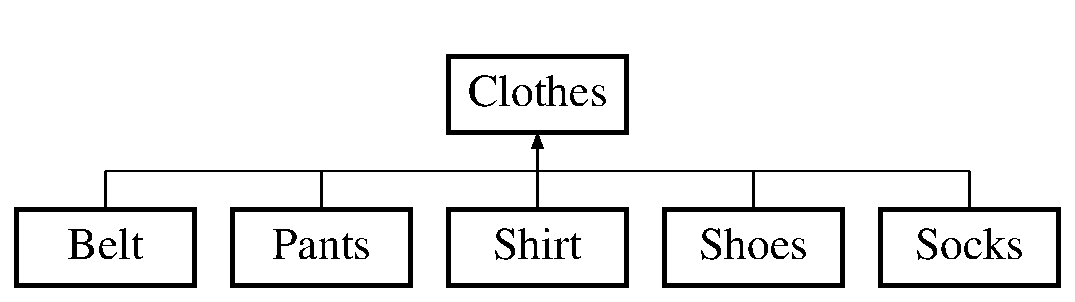
\includegraphics[height=2.000000cm]{classClothes}
\end{center}
\end{figure}
\subsection*{Public Member Functions}
\begin{DoxyCompactItemize}
\item 
\mbox{\Hypertarget{classClothes_a3f6dac172f333126d19010f85ec44e4c}\label{classClothes_a3f6dac172f333126d19010f85ec44e4c}} 
int {\bfseries Get\+ID} ()
\item 
\mbox{\Hypertarget{classClothes_a48787b979453e916476a28f703802d23}\label{classClothes_a48787b979453e916476a28f703802d23}} 
string {\bfseries Parm\+Name} (string name=name\+\_\+)
\item 
\mbox{\Hypertarget{classClothes_a0ee1ffc9971a7bdea45dac35808e168b}\label{classClothes_a0ee1ffc9971a7bdea45dac35808e168b}} 
string {\bfseries Parm\+Prim\+Color} (string color=primary\+\_\+color\+\_\+)
\item 
\mbox{\Hypertarget{classClothes_a15a02c1fae95353d0d0b91694df70b61}\label{classClothes_a15a02c1fae95353d0d0b91694df70b61}} 
string {\bfseries Parm\+Sec\+Color} (string color=secondary\+\_\+color\+\_\+)
\item 
\mbox{\Hypertarget{classClothes_ae6fc82beb6598ddfb2fc5e3253c55d8c}\label{classClothes_ae6fc82beb6598ddfb2fc5e3253c55d8c}} 
string {\bfseries Parm\+Tert\+Color} (string color=tertiary\+\_\+color\+\_\+)
\item 
\mbox{\Hypertarget{classClothes_a44f5372b75126d966c259cad7c0de4b3}\label{classClothes_a44f5372b75126d966c259cad7c0de4b3}} 
string {\bfseries Parm\+Pattern} (string pattern=pattern\+\_\+)
\item 
\mbox{\Hypertarget{classClothes_a02f6501724c1001227e35c46424e248a}\label{classClothes_a02f6501724c1001227e35c46424e248a}} 
string {\bfseries Parm\+Material} (string material=material\+\_\+)
\item 
\mbox{\Hypertarget{classClothes_a58f99417f81e5d31ff90cbc830dce314}\label{classClothes_a58f99417f81e5d31ff90cbc830dce314}} 
string {\bfseries Parm\+Style} (string style=style\+\_\+)
\item 
\mbox{\Hypertarget{classClothes_a5b8d63002853915190cdf7d8d94a1f6a}\label{classClothes_a5b8d63002853915190cdf7d8d94a1f6a}} 
string {\bfseries Parm\+Length} (string length=length\+\_\+)
\item 
\mbox{\Hypertarget{classClothes_a63123eab288649126464d2f8944a0be1}\label{classClothes_a63123eab288649126464d2f8944a0be1}} 
string {\bfseries Parm\+Cut} (string cut=cut\+\_\+)
\item 
\mbox{\Hypertarget{classClothes_ad568215e8c1751e45438d67c87f05361}\label{classClothes_ad568215e8c1751e45438d67c87f05361}} 
string {\bfseries Parm\+Sleeve\+Length} (string length=length\+\_\+)
\item 
\mbox{\Hypertarget{classClothes_abb6030ba8b16e1f6155a8697d3386311}\label{classClothes_abb6030ba8b16e1f6155a8697d3386311}} 
string {\bfseries Parm\+Collar} (string collar=collar\+\_\+)
\item 
\mbox{\Hypertarget{classClothes_a953d143394e9a2c007ab0c3a638973cf}\label{classClothes_a953d143394e9a2c007ab0c3a638973cf}} 
virtual string {\bfseries To\+String} () const =0
\end{DoxyCompactItemize}
\subsection*{Protected Attributes}
\begin{DoxyCompactItemize}
\item 
\mbox{\Hypertarget{classClothes_a8978d931db5ca47c3ccea30def4ae83e}\label{classClothes_a8978d931db5ca47c3ccea30def4ae83e}} 
int {\bfseries id\+\_\+} = k\+Dummy\+ID
\item 
\mbox{\Hypertarget{classClothes_a7f2275aaae24224d60c48af922c31b65}\label{classClothes_a7f2275aaae24224d60c48af922c31b65}} 
string {\bfseries name\+\_\+} = k\+Dummy\+Name
\item 
\mbox{\Hypertarget{classClothes_a7cb005bf6cbb7f4eaa40f1b31817559c}\label{classClothes_a7cb005bf6cbb7f4eaa40f1b31817559c}} 
string {\bfseries primary\+\_\+color\+\_\+} = k\+Dummy\+Prim\+Color
\item 
\mbox{\Hypertarget{classClothes_ab8f55f67b956b25d71260cffcf273673}\label{classClothes_ab8f55f67b956b25d71260cffcf273673}} 
string {\bfseries secondary\+\_\+color\+\_\+} = k\+Dummy\+Sec\+Color
\item 
\mbox{\Hypertarget{classClothes_a3c5f1e7ab531e3ba7a38b930da8078a0}\label{classClothes_a3c5f1e7ab531e3ba7a38b930da8078a0}} 
string {\bfseries tertiary\+\_\+color\+\_\+} = k\+Dummy\+Tert\+Color
\item 
\mbox{\Hypertarget{classClothes_a1d40145a4eb6d28441f112f030ab5d35}\label{classClothes_a1d40145a4eb6d28441f112f030ab5d35}} 
string {\bfseries pattern\+\_\+} = k\+Dummy\+Pattern
\item 
\mbox{\Hypertarget{classClothes_adbb9ed311f14ccbb1e4fe0e8378a95d4}\label{classClothes_adbb9ed311f14ccbb1e4fe0e8378a95d4}} 
string {\bfseries material\+\_\+} = k\+Dummy\+Material
\item 
\mbox{\Hypertarget{classClothes_aa85ed2b95110d8c477a1aca9cb403f98}\label{classClothes_aa85ed2b95110d8c477a1aca9cb403f98}} 
string {\bfseries style\+\_\+} = k\+Dummy\+Style
\item 
\mbox{\Hypertarget{classClothes_ae02603eda727e33caf46ec30e761e3c3}\label{classClothes_ae02603eda727e33caf46ec30e761e3c3}} 
string {\bfseries length\+\_\+} = k\+Dummy\+Length
\item 
\mbox{\Hypertarget{classClothes_ac1c2286c8928a5eee91d818a098a44ac}\label{classClothes_ac1c2286c8928a5eee91d818a098a44ac}} 
string {\bfseries cut\+\_\+} = k\+Dummy\+Cut
\item 
\mbox{\Hypertarget{classClothes_a012aeb71e62ebaf9b5b5dd700cc8d5db}\label{classClothes_a012aeb71e62ebaf9b5b5dd700cc8d5db}} 
string {\bfseries sleeve\+\_\+length\+\_\+} = k\+Dummy\+Sleeve\+Length
\item 
\mbox{\Hypertarget{classClothes_ae2e5026257b3a2f2ddbf61757fd3b57b}\label{classClothes_ae2e5026257b3a2f2ddbf61757fd3b57b}} 
string {\bfseries collar\+\_\+} = k\+Dummy\+Collar
\end{DoxyCompactItemize}


The documentation for this class was generated from the following file\+:\begin{DoxyCompactItemize}
\item 
clothes.\+h\end{DoxyCompactItemize}

\hypertarget{classPants}{}\section{Pants Class Reference}
\label{classPants}\index{Pants@{Pants}}
Inheritance diagram for Pants\+:\begin{figure}[H]
\begin{center}
\leavevmode
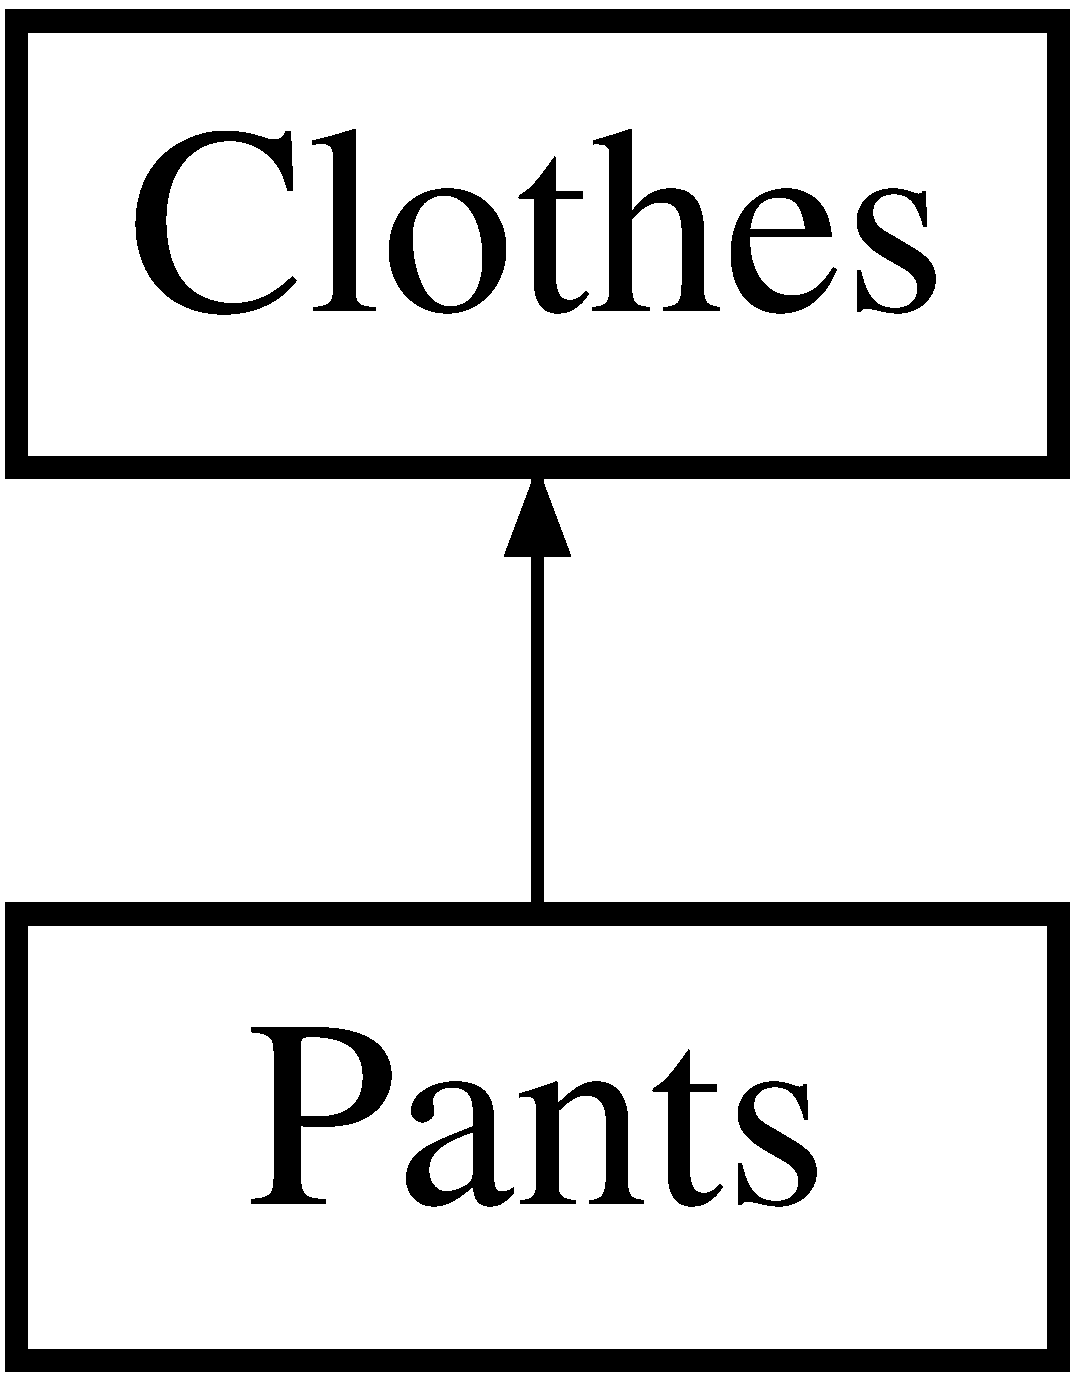
\includegraphics[height=2.000000cm]{classPants}
\end{center}
\end{figure}
\subsection*{Public Member Functions}
\begin{DoxyCompactItemize}
\item 
\mbox{\Hypertarget{classPants_a9ca6f6ddce0ac46556b6e56a9d73ddd0}\label{classPants_a9ca6f6ddce0ac46556b6e56a9d73ddd0}} 
{\bfseries Pants} (int id, string name, string prim\+\_\+color, string sec\+\_\+color, string tert\+\_\+color, string material, string length, string cut)
\item 
\mbox{\Hypertarget{classPants_aa62270b70cbb40b7b420f1091ad7e43b}\label{classPants_aa62270b70cbb40b7b420f1091ad7e43b}} 
string {\bfseries To\+X\+ML} () const
\item 
\mbox{\Hypertarget{classPants_a9b5fcde766a77877bf428e18c65f1e70}\label{classPants_a9b5fcde766a77877bf428e18c65f1e70}} 
string {\bfseries To\+String} () const
\end{DoxyCompactItemize}
\subsection*{Additional Inherited Members}


The documentation for this class was generated from the following files\+:\begin{DoxyCompactItemize}
\item 
pants.\+h\item 
pants.\+cc\end{DoxyCompactItemize}

\hypertarget{classShirt}{}\section{Shirt Class Reference}
\label{classShirt}\index{Shirt@{Shirt}}
Inheritance diagram for Shirt\+:\begin{figure}[H]
\begin{center}
\leavevmode
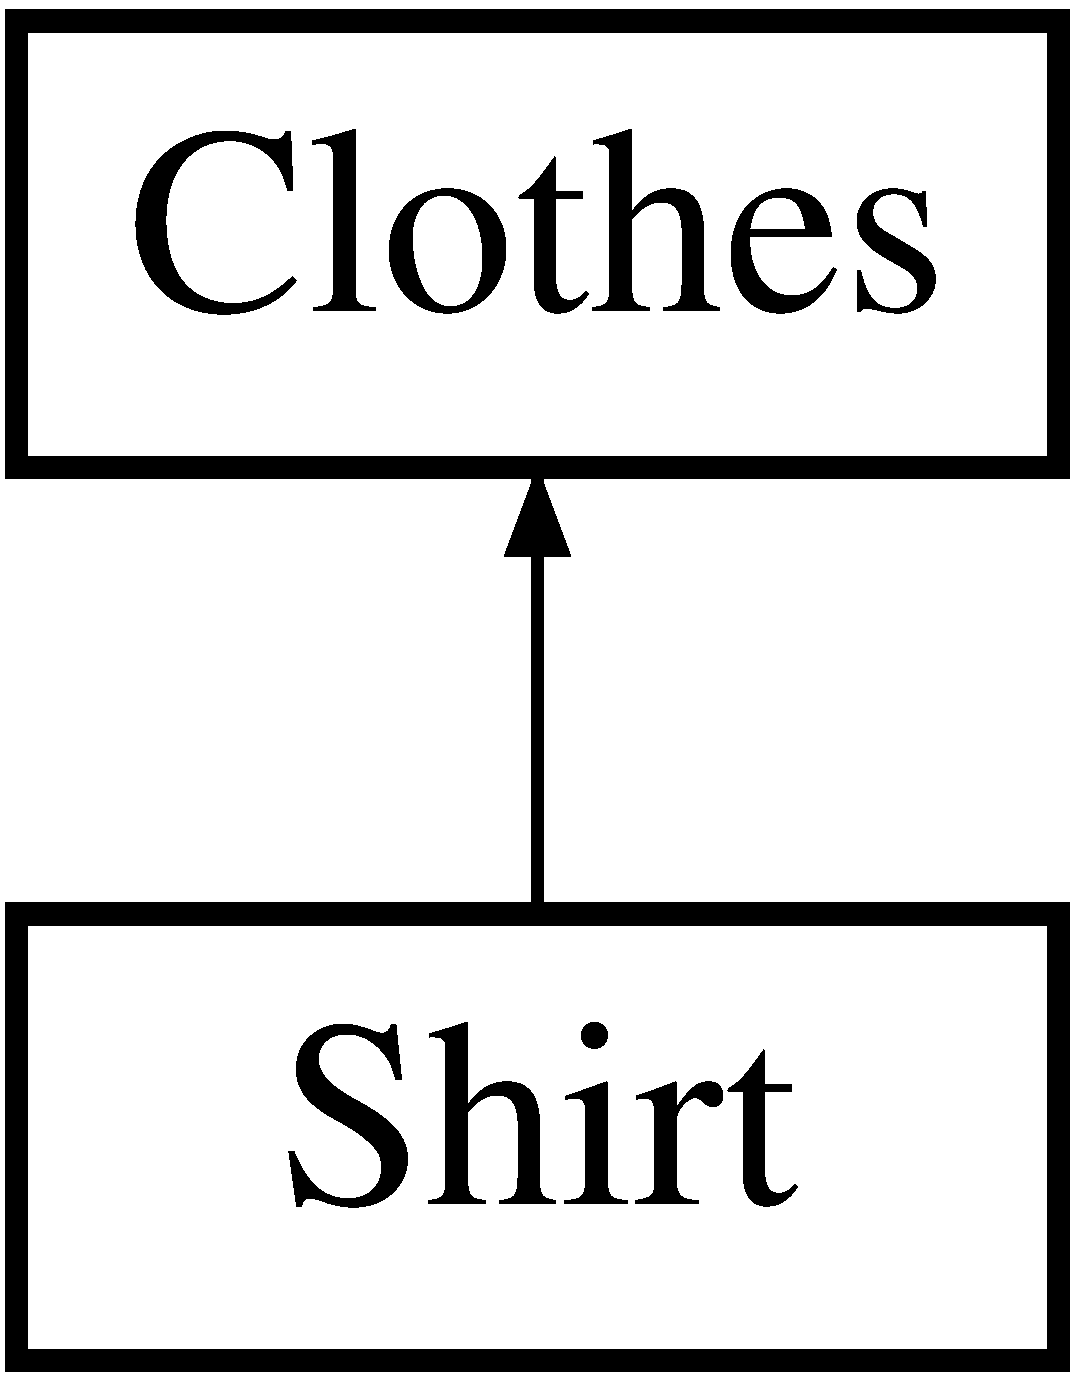
\includegraphics[height=2.000000cm]{classShirt}
\end{center}
\end{figure}
\subsection*{Public Member Functions}
\begin{DoxyCompactItemize}
\item 
\mbox{\Hypertarget{classShirt_a5df3975569b7f5874a905d31e4056b7b}\label{classShirt_a5df3975569b7f5874a905d31e4056b7b}} 
{\bfseries Shirt} (int id, string name, string prim\+\_\+color, string sec\+\_\+color, string tert\+\_\+color, string pattern, string sleeve\+\_\+length, string collar)
\item 
\mbox{\Hypertarget{classShirt_ae636e58135bd1ca4ac590e55e8d47cac}\label{classShirt_ae636e58135bd1ca4ac590e55e8d47cac}} 
string {\bfseries To\+X\+ML} () const
\item 
\mbox{\Hypertarget{classShirt_ab85aaa20a603d63f4144d1b42d9b616d}\label{classShirt_ab85aaa20a603d63f4144d1b42d9b616d}} 
string {\bfseries To\+String} () const
\end{DoxyCompactItemize}
\subsection*{Additional Inherited Members}


The documentation for this class was generated from the following files\+:\begin{DoxyCompactItemize}
\item 
shirt.\+h\item 
shirt.\+cc\end{DoxyCompactItemize}

\hypertarget{classShoes}{}\section{Shoes Class Reference}
\label{classShoes}\index{Shoes@{Shoes}}
Inheritance diagram for Shoes\+:\begin{figure}[H]
\begin{center}
\leavevmode
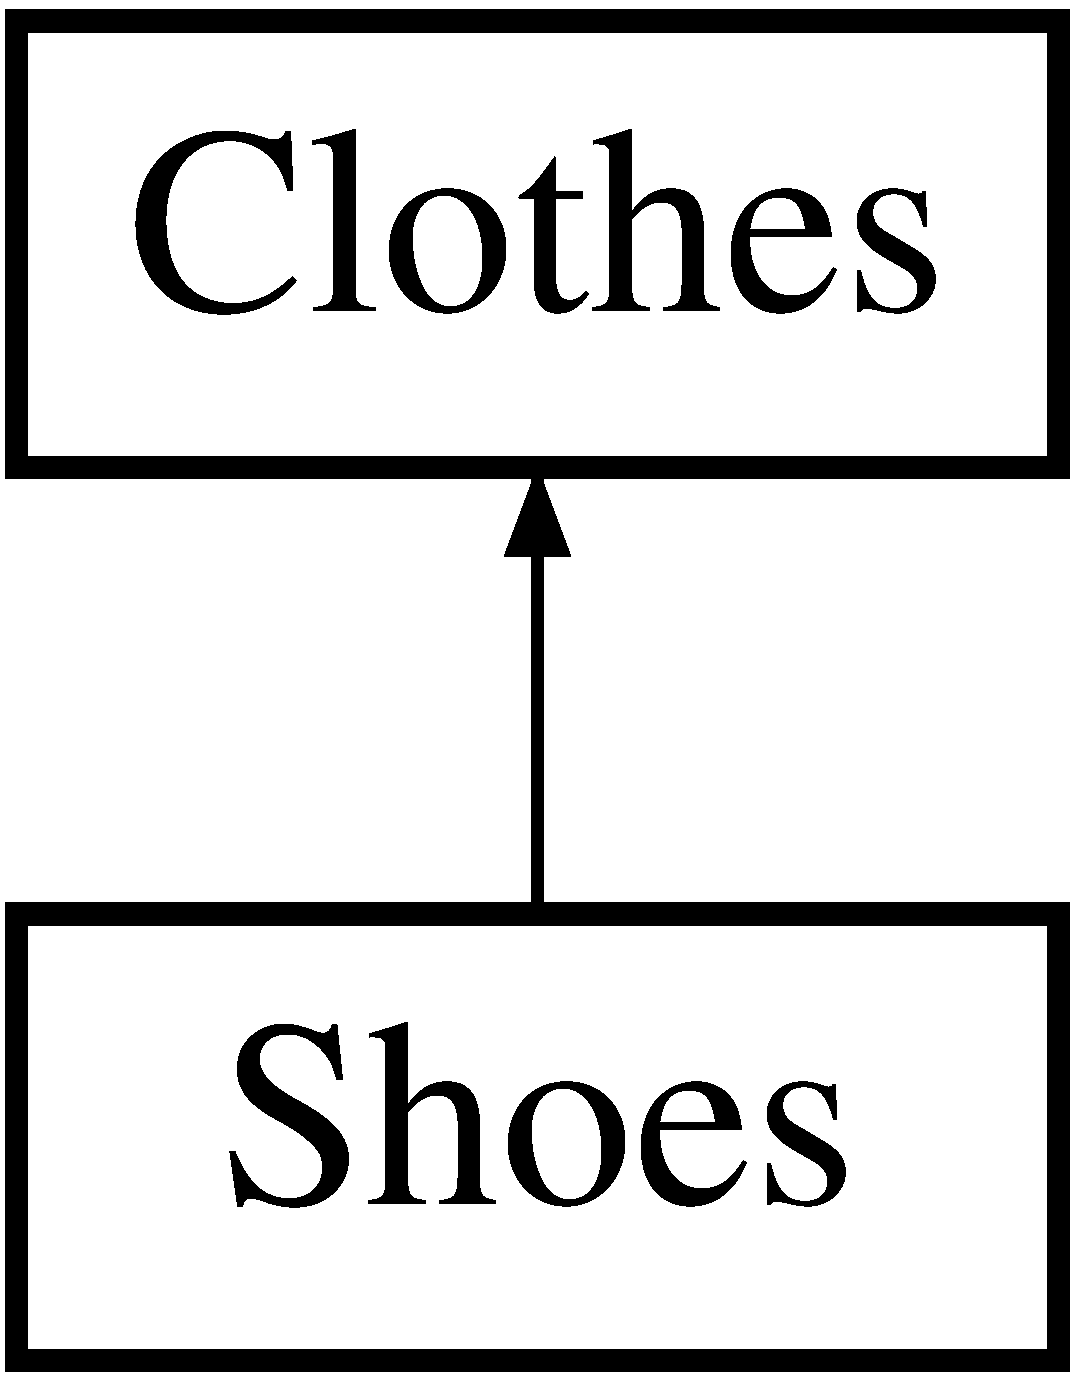
\includegraphics[height=2.000000cm]{classShoes}
\end{center}
\end{figure}
\subsection*{Public Member Functions}
\begin{DoxyCompactItemize}
\item 
\mbox{\Hypertarget{classShoes_a4f38fcd11c63cf3256c9688cf1bd19b3}\label{classShoes_a4f38fcd11c63cf3256c9688cf1bd19b3}} 
{\bfseries Shoes} (int id, string name, string prim\+\_\+color, string sec\+\_\+color, string tert\+\_\+color, string material, string style)
\item 
\mbox{\Hypertarget{classShoes_acf6f049aa995a189b0f892f86defeefd}\label{classShoes_acf6f049aa995a189b0f892f86defeefd}} 
string {\bfseries To\+X\+ML} () const
\item 
\mbox{\Hypertarget{classShoes_a9b1bcc00ec7ef920d34bf9193c96a1ce}\label{classShoes_a9b1bcc00ec7ef920d34bf9193c96a1ce}} 
string {\bfseries To\+String} () const
\end{DoxyCompactItemize}
\subsection*{Additional Inherited Members}


The documentation for this class was generated from the following files\+:\begin{DoxyCompactItemize}
\item 
shoes.\+h\item 
shoes.\+cc\end{DoxyCompactItemize}

\hypertarget{classSocks}{}\section{Socks Class Reference}
\label{classSocks}\index{Socks@{Socks}}
Inheritance diagram for Socks\+:\begin{figure}[H]
\begin{center}
\leavevmode
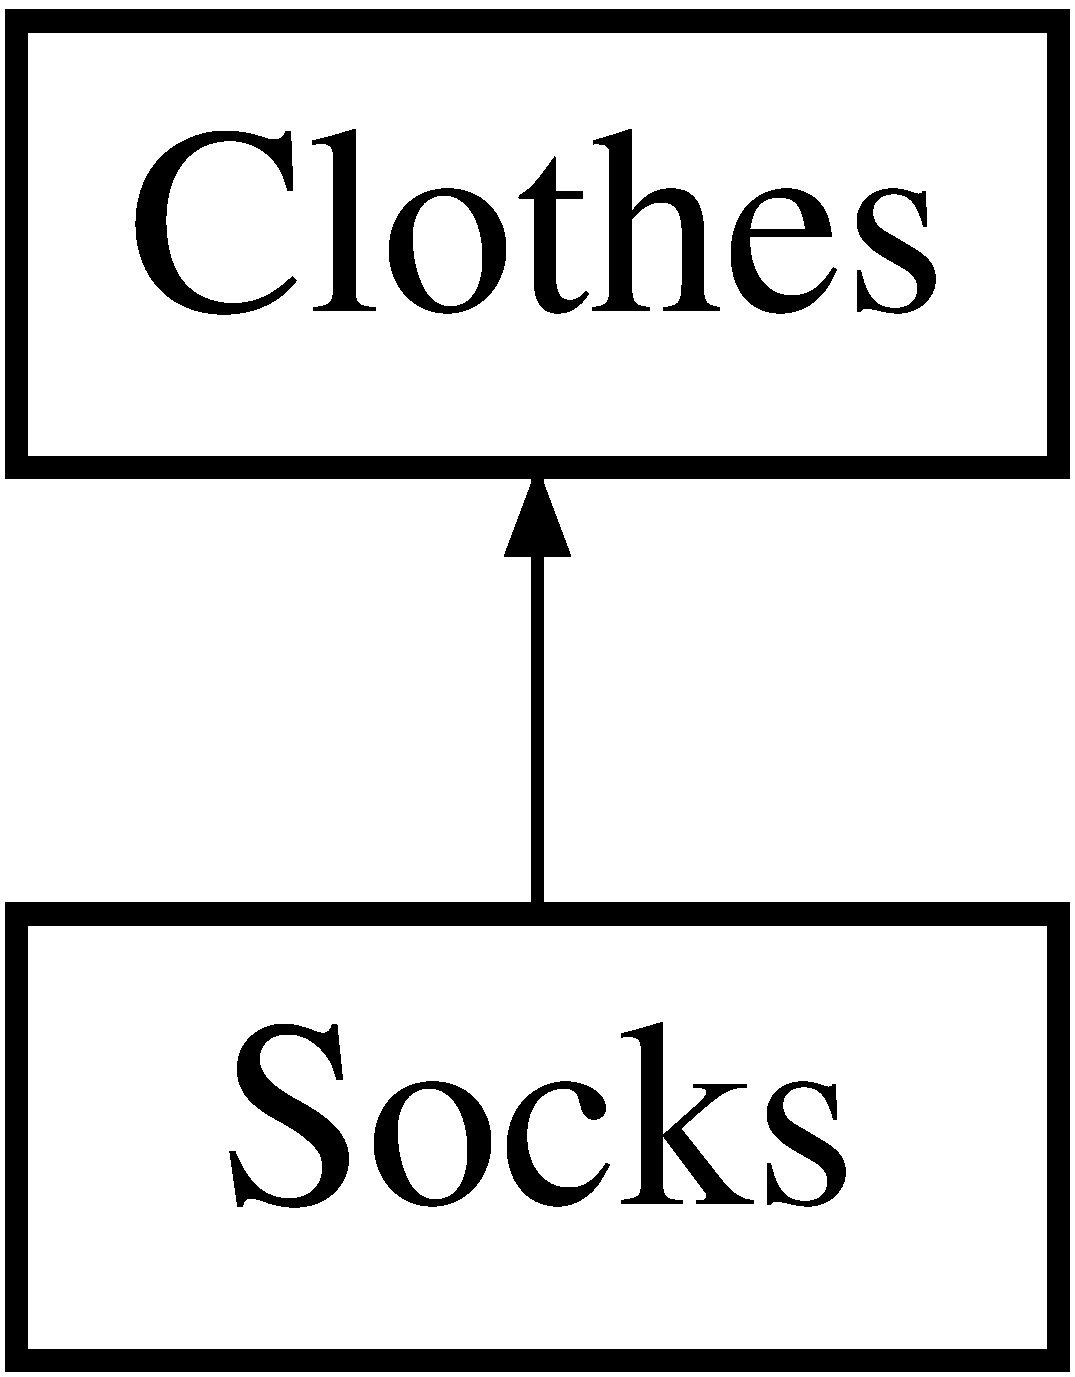
\includegraphics[height=2.000000cm]{classSocks}
\end{center}
\end{figure}
\subsection*{Public Member Functions}
\begin{DoxyCompactItemize}
\item 
\mbox{\Hypertarget{classSocks_ab8f83e88b6131bbf22d75de7a41d241a}\label{classSocks_ab8f83e88b6131bbf22d75de7a41d241a}} 
{\bfseries Socks} (int id, string name, string prim\+\_\+color, string sec\+\_\+color, string tert\+\_\+color, string pattern)
\item 
\mbox{\Hypertarget{classSocks_a5ecf1671277183b60f8eea7020cf32ed}\label{classSocks_a5ecf1671277183b60f8eea7020cf32ed}} 
string {\bfseries To\+X\+ML} () const
\item 
\mbox{\Hypertarget{classSocks_aad237fbcc4ccf36a2956fcdef8760683}\label{classSocks_aad237fbcc4ccf36a2956fcdef8760683}} 
string {\bfseries To\+String} () const
\end{DoxyCompactItemize}
\subsection*{Additional Inherited Members}


The documentation for this class was generated from the following files\+:\begin{DoxyCompactItemize}
\item 
socks.\+h\item 
socks.\+cc\end{DoxyCompactItemize}

\hypertarget{classVulkan}{}\section{Vulkan Class Reference}
\label{classVulkan}\index{Vulkan@{Vulkan}}
Inheritance diagram for Vulkan\+:\begin{figure}[H]
\begin{center}
\leavevmode
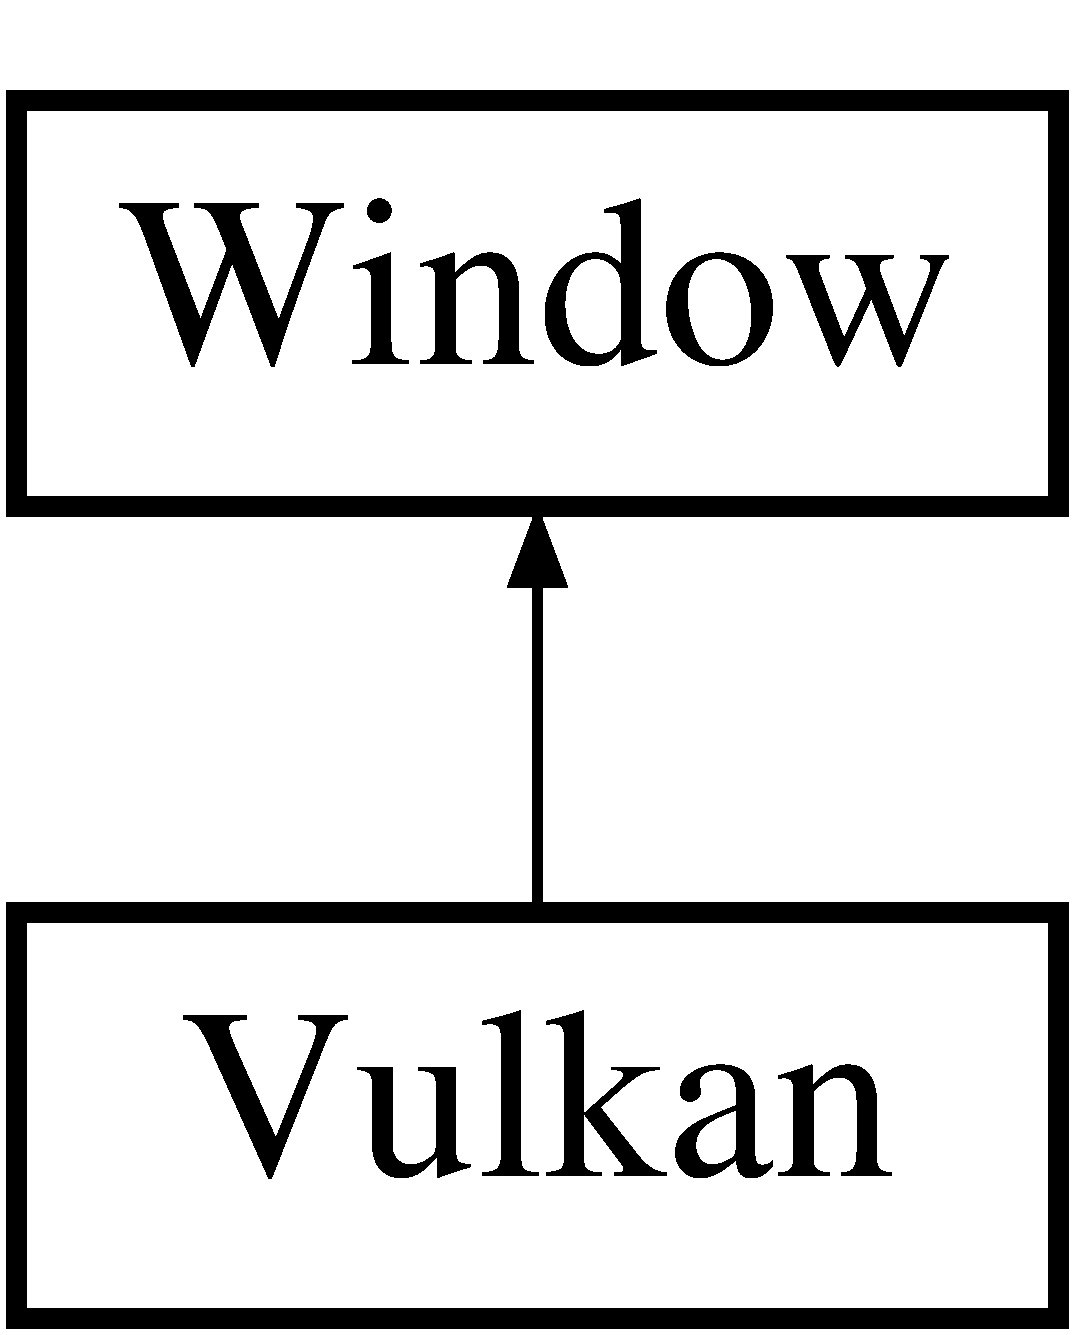
\includegraphics[height=2.000000cm]{classVulkan}
\end{center}
\end{figure}
\subsection*{Additional Inherited Members}


The documentation for this class was generated from the following file\+:\begin{DoxyCompactItemize}
\item 
vulkan.\+h\end{DoxyCompactItemize}

\hypertarget{classWindow}{}\section{Window Class Reference}
\label{classWindow}\index{Window@{Window}}
Inheritance diagram for Window\+:\begin{figure}[H]
\begin{center}
\leavevmode
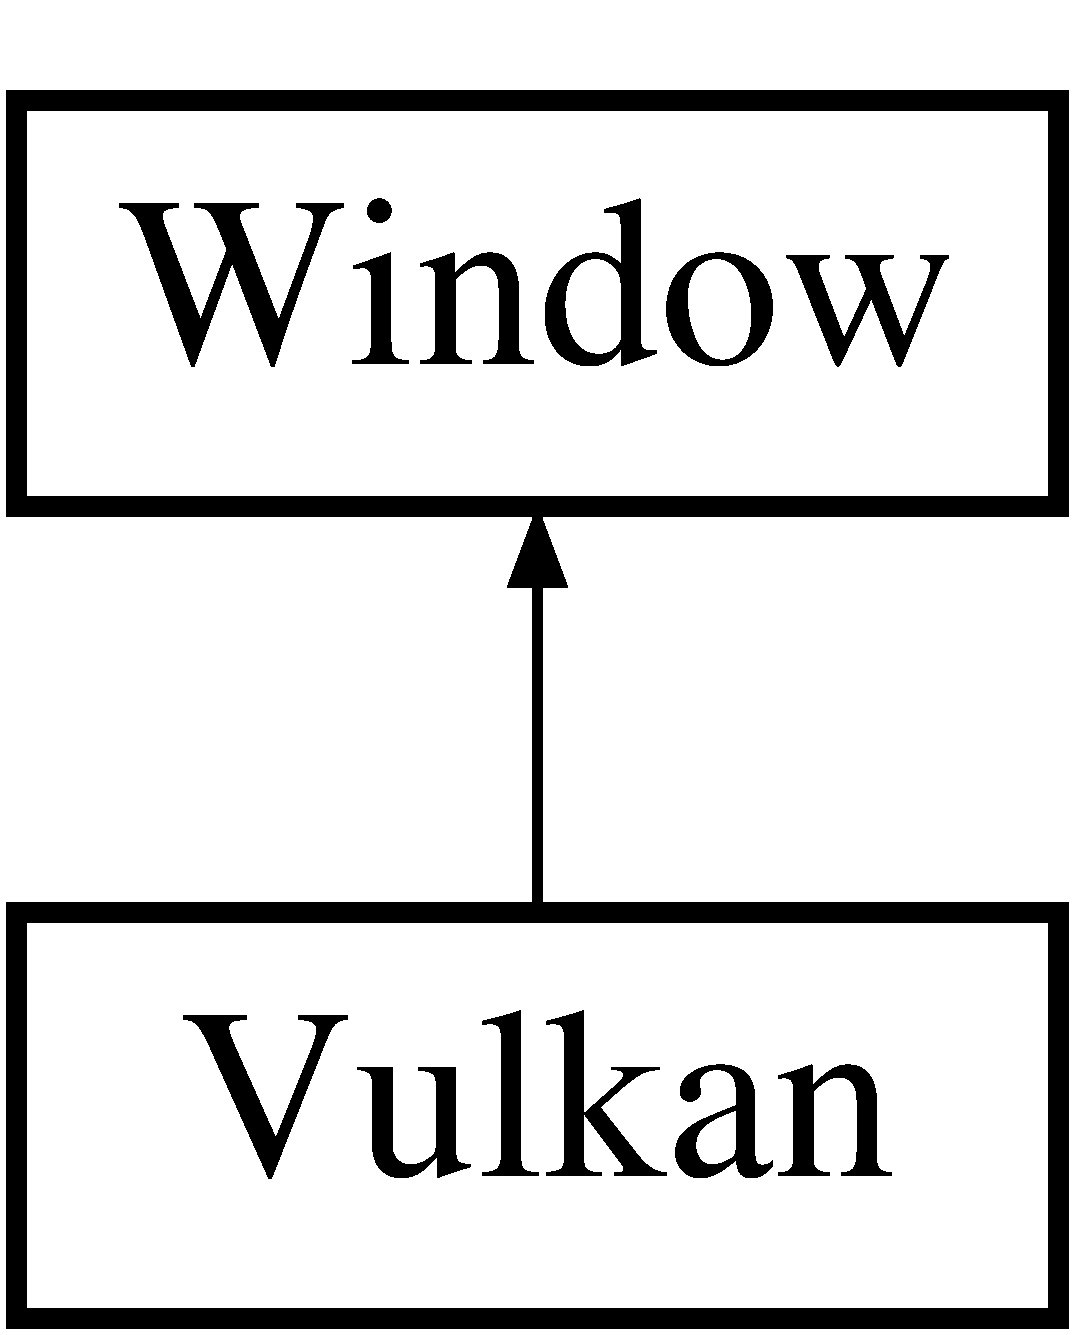
\includegraphics[height=2.000000cm]{classWindow}
\end{center}
\end{figure}
\subsection*{Public Member Functions}
\begin{DoxyCompactItemize}
\item 
\mbox{\Hypertarget{classWindow_a81a8bcd04b0b760f5616893c318bb705}\label{classWindow_a81a8bcd04b0b760f5616893c318bb705}} 
bool {\bfseries Init} ()
\item 
\mbox{\Hypertarget{classWindow_a1da23fba0fda380329f20484244814e1}\label{classWindow_a1da23fba0fda380329f20484244814e1}} 
void {\bfseries Die} ()
\item 
\mbox{\Hypertarget{classWindow_a839fb7e78dd72784f6ed8097131d9e9e}\label{classWindow_a839fb7e78dd72784f6ed8097131d9e9e}} 
char {\bfseries Window\+Char} ()
\end{DoxyCompactItemize}


The documentation for this class was generated from the following file\+:\begin{DoxyCompactItemize}
\item 
window.\+h\end{DoxyCompactItemize}

%--- End generated contents ---

% Index
\backmatter
\newpage
\phantomsection
\clearemptydoublepage
\addcontentsline{toc}{chapter}{Index}
\printindex

\end{document}
